% ============================================================
%  第六部分：历史实证
% ============================================================

\section{历史实证：黑色系产业链的状态演化}
\label{sec:empirical}

前面全部论述最终要接受数据的检验。本章用真实期货数据完成三个实证任务：（一）产业链状态的演化复盘；（二）切换统计与检测粒度；（三）条件化口径与静态口径的对比。所有结果均可由随附脚本严格因果地复现，未对生产系统的识别逻辑做任何参数修改。

\subsection{实验设计}

\subsubsection{对象、数据与方法}

\begin{itemize}[itemsep=2pt]
\item \textbf{对象}：黑色系产业链（RB 螺纹、HC 热卷、I 铁矿、J 焦炭、JM 焦煤、FG 玻璃、SF 硅铁、SM 锰硅）；
\item \textbf{数据}：本地 DuckDB 主力连续日线（含持仓量），各品种共同可得区间约 2019-11 至 2026-08，六个完整年度；
\item \textbf{合成指数}：首日归一化 $+$ 等权平均（与生产系统一致）；
\item \textbf{识别方法}：完整复用生产系统的 L2 识别器（五状态高斯 HMM 三窗口投票 $+$ 规则法合成 $+$ 驱动力识别）。
\end{itemize}

\subsubsection{严格因果的 walk-forward 协议}

实证的核心纪律是把第二章的“滤波原则”贯彻到每一行代码：

\begin{enumerate}[itemsep=2pt]
\item 以每 10 个交易日为一个决策日；
\item 每个决策日 $t$：合成指数与全部成员数据都截断到 $t$（成员截断尤其关键——驱动力与分散度指标只允许看到截至当日的趋势）；
\item 由 $t$ 日可见数据重新训练 HMM（三窗口 $\times$ 五个随机初始化）并完成状态判定；
\item 状态在 $t$ 日产生、$t+1$ 日起生效，一直维持到下一个决策日——这正是实时系统的真实行为。
\end{enumerate}

\begin{remark}[关于 10 日粒度的诚实声明]
每 10 个交易日回看一次是计算成本与演示清晰度的折中（生产系统可以按日运行）。这一粒度本身构成“量化延迟”的一部分：即便识别器立即判定切换，状态信号最早也只能在下一个决策日更新——因此本章测量的所有“切换时点”都带有至多 10 个交易日的额外粒度延迟。把它显式声明出来，胜过在结果中假装拥有日度分辨率。
\end{remark}

\subsection{案例一：状态演化复盘}

按上述协议得到的完整状态序列如图~\ref{fig:l2-evolution} 所示。六个年度中，状态序列呈现出三段截然不同的形态：

\begin{itemize}[itemsep=2pt]
\item \textbf{2021 年：高频切换期}。政策调控与商品暴涨暴跌交替，状态在牛市/熊市/高波动之间快速轮换（单步即翻转的区间密集出现），是典型的“转折点密集”环境；
\item \textbf{2022--2024 年：震荡主导期}。震荡与低波动交替，间以若干段高波动（如 2022 年上半年）——黑色系整体进入无趋势状态；
\item \textbf{2025--2026 年：长沉睡期}。自 2025 年 9 月至 2026 年 3 月出现全程最长的一段连续震荡（约 200 个自然日），情绪与波动双低。
\end{itemize}

\begin{figure}[htbp]
\centering
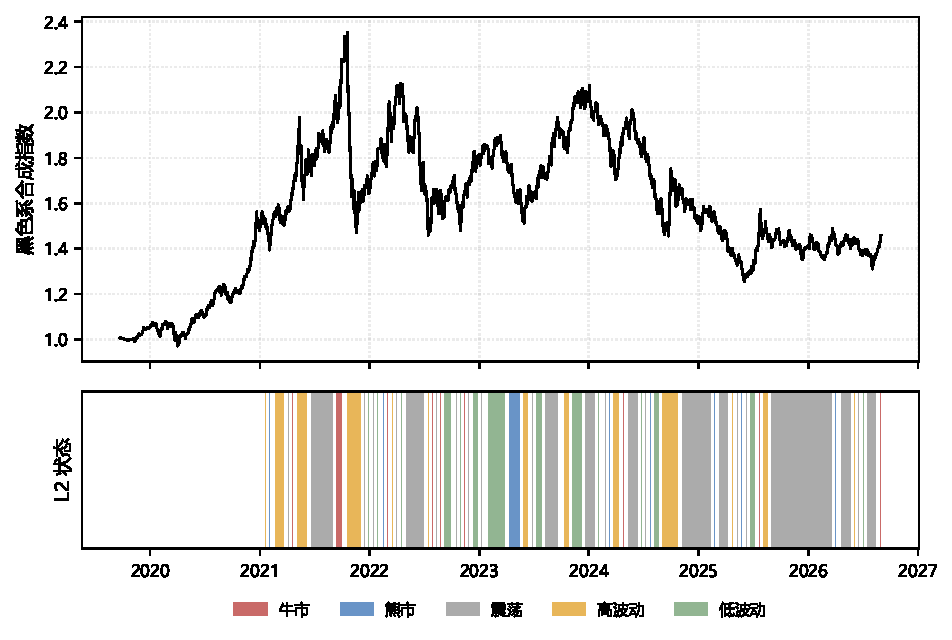
\includegraphics[width=\linewidth]{figures/fig_l2_evolution.pdf}
\caption{黑色系产业链 L2 状态演化（walk-forward 回看，每 10 个交易日重估；色带为状态，上图为合成指数）}
\label{fig:l2-evolution}
\end{figure}

\subsection{案例二：切换统计与检测粒度}

多次回看的区间折叠后得到 68 个状态区间、67 次切换（六年样本，平均约每 37 个自然日一次切换）。各状态的画像与持续期结构如表~\ref{tab:l2-stats} 与图~\ref{fig:l2-stats} 所示。

\begin{table}[htbp]
\centering
\footnotesize
\begin{tabular}{lccccc}
\toprule
\textbf{状态} & \textbf{占比} & \textbf{平均持续期（天）} & \textbf{最长（天）} & \textbf{区间数} & \textbf{平均置信度} \\
\midrule
震荡 & 47.4\% & 25.4 & 200 & 24 & 0.70 \\
高波动 & 19.7\% & 15.9 & 51 & 13 & 0.69 \\
低波动 & 18.2\% & 11.2 & 56 & 14 & 0.65 \\
熊市 & 7.3\% & 4.1 & 33 & 8 & 0.53 \\
牛市 & 7.3\% & 1.8 & 16 & 9 & 0.55 \\
\bottomrule
\end{tabular}
\caption{黑色系 L2 状态画像（2019-11 至 2026-08，137 个决策步）}
\label{tab:l2-stats}
\end{table}

\begin{figure}[htbp]
\centering
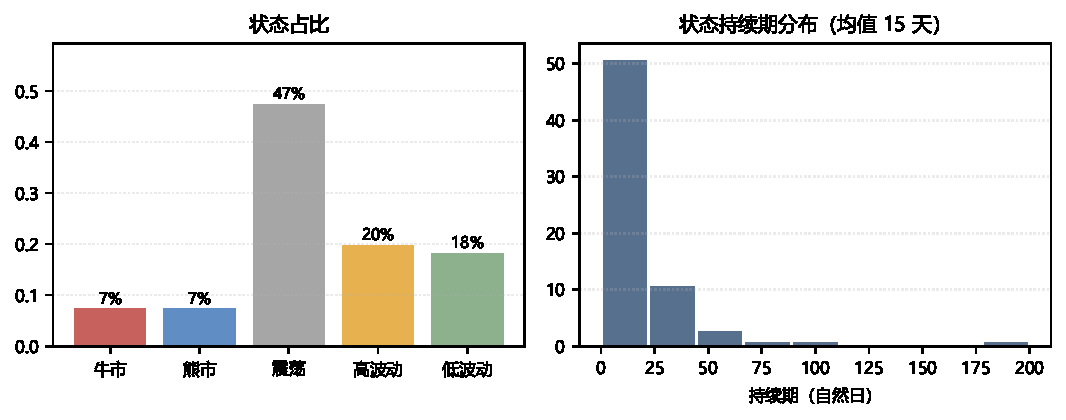
\includegraphics[width=\linewidth]{figures/fig_l2_stats.pdf}
\caption{各状态占比（左）与状态持续期分布（右）}
\label{fig:l2-stats}
\end{figure}

三个值得诚实讨论的发现：

\begin{enumerate}[itemsep=3pt]
\item \textbf{牛/熊是“短促状态”，震荡/波动是常态}。牛市平均仅持续 1.8 个自然日、熊市 4.1 天，而震荡 25.4 天——黑色系在样本期内大部分时间并不存在可持续的“方向性状态”。这直接呼应第一部分的信息论下界：\emph{持续期越短的状态，与噪声在统计上越难区分}；识别器对牛/熊判定给出的平均置信度（$0.53$/$0.55$）也确实低于震荡/高波（$0.65$--$0.70$）——系统的输出与状态的统计现实是自洽的。
\item \textbf{切换频率不低}。六年 67 次切换、年化换手 6.6 倍（条件化口径），说明该系统的自然工作点偏向“敏感”一侧。对成本高度敏感的场景，应把阈值/确认机制向“迟钝”方向调整——这正是第一部分“工作点选择”的工程含义。
\item \textbf{量化延迟的构成}。探到的每个切换时点都包含三层延迟：数据层面（日线收盘可见）、识别层面（HMM 窗口投票的确认）、粒度层面（实证为 10 个交易日）。生产系统消除第三层后可接近日度分辨率，但前两层由统计下界决定，不可消除。
\end{enumerate}

\subsection{案例三：条件化口径与静态口径}

用状态序列驱动一个演示性暴露规则（牛市 $+1$、低波动 $+0.5$、震荡/高波动 $0$、熊市 $-1$；$t$ 日决策、$t+1$ 日生效；单边成本 5\,bps），与买入持有对比，结果如表~\ref{tab:l2-conditional} 与图~\ref{fig:l2-conditional}。

\begin{table}[htbp]
\centering
\footnotesize
\begin{tabular}{lcccccc}
\toprule
\textbf{口径} & \textbf{累计收益} & \textbf{年化收益} & \textbf{年化波动} & \textbf{Sharpe} & \textbf{最大回撤} & \textbf{年换手} \\
\midrule
状态条件化 & 45.0\% & 6.4\% & 11.0\% & 0.56 & $-18.3\%$ & 6.6$\times$ \\
买入持有 & 44.9\% & 8.6\% & 23.3\% & 0.35 & $-46.7\%$ & 0$\times$ \\
\bottomrule
\end{tabular}
\caption{条件化口径与买入持有的对比（演示设定：1 日延迟、单边 5\,bps）}
\label{tab:l2-conditional}
\end{table}

\begin{figure}[htbp]
\centering
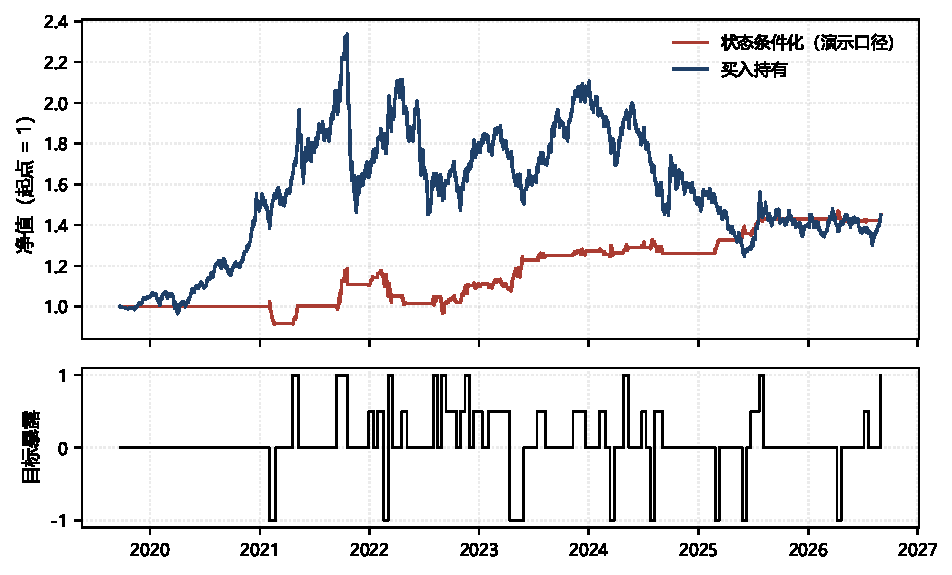
\includegraphics[width=\linewidth]{figures/fig_l2_conditional.pdf}
\caption{条件化口径与买入持有的净值曲线（上）与目标暴露（下，阶梯线）}
\label{fig:l2-conditional}
\end{figure}

结果给出的最重要事实，恰恰\textbf{不是}“条件化跑赢了”，而是：

\begin{itemize}[itemsep=2pt]
\item \textbf{收益中枢几乎不变}（累计 45.0\% vs 44.9\%）——条件化没有、也不应该被期待“创造收益”；
\item \textbf{风险特征近对折}：年化波动率 23.3\% $\to$ 11.0\%，最大回撤 $-46.7\%$ $\to$ $-18.3\%$，Sharpe 从 0.35 提升到 0.56；
\item \textbf{代价是换手}：6.6 倍年换手意味着在更高成本假设（如 15--20\,bps 单边）或流动性约束下，优势会被显著侵蚀——把成本敏感性测试列为必做项，而非可选。
\end{itemize}

这个形态（\emph{收益持平、风险减半}）与第五部分对前沿文献的批判性综合（“价值在风险特征与实施稳健性”）完全一致，是理论与实证之间最有力的交叉验证。

\subsection{发现的诚实汇总}

把三个案例放回理论框架，得到三处呼应，以及必须同时声明的边界：

\begin{enumerate}[itemsep=3pt]
\item \textbf{呼应一（价值定位）}：条件化未提升收益中枢，却在波动与回撤上取得近似减半的改善——系统价值位于风险端。这与信息论下界一致：识别无法“看得更远”，但足以“守得更稳”。
\item \textbf{呼应二（下界现实）}：牛/熊状态的短促持续期与较低置信度，是状态本身接近统计不可检测的直接体现；系统的保守判定（多窗口投票）是对这一现实的正确工程响应。
\item \textbf{呼应三（成本与工作点）}：67 次切换与 6.6$\times$ 换手提示当前工作点偏敏感；面向成本敏感场景，应向“确认更慢、误报更少”方向调整，并接受由此增大的检测延迟。
\item \textbf{边界声明}：本实证覆盖\emph{单一产业链、单一样本区间}（含疫情、地产周期等特殊结构），条件化暴露为\emph{演示性映射}而非策略推荐；结论的效度限于“方法论流程可复现、理论判断可被数据呼应”这两层，不外推为策略有效性证明。
\end{enumerate}